\subsection*{Analysis Common File Types}
\label{sec:analysisCommonFileTypes}

\begin{figure}[H]
    \centering
    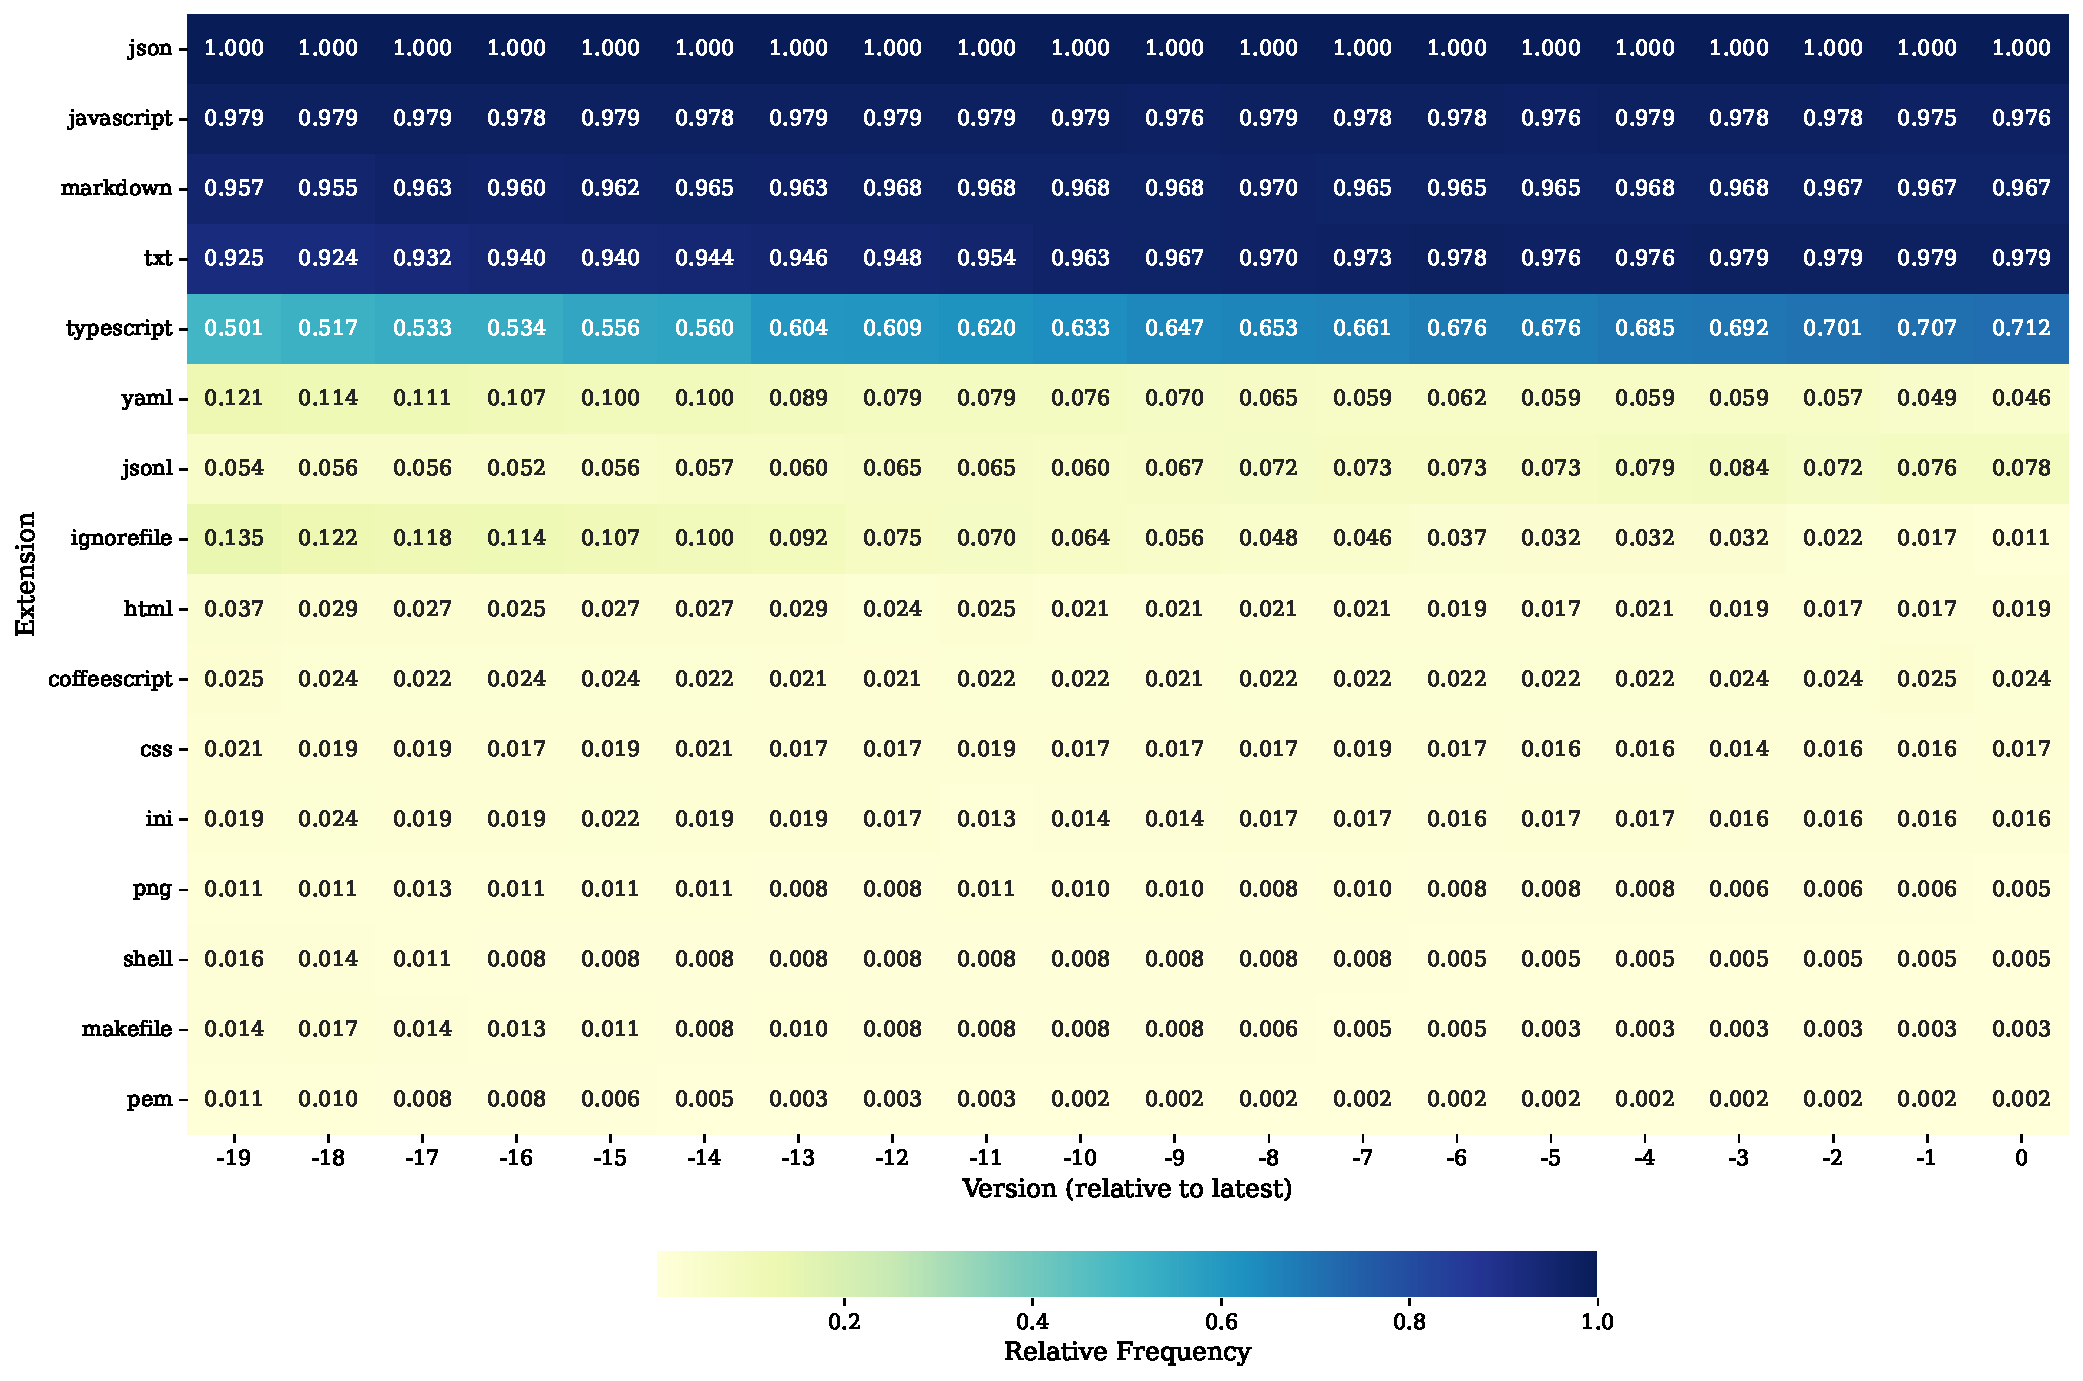
\includegraphics[width=\textwidth]{metrics/filetype/heatmap_common.pdf}
    \caption{Heatmap For Common File Types}
    \label{fig:fig1ComFileTypes}
\end{figure}

From \cref{fig:fig1ComFileTypes}, we can observe that:
\begin{itemize}
    \item 
    At least one JSON file is always present in all packages across all versions.
    This is because an \ac{NPM} package must contain a \texttt{package.json} file in order to be published to the \ac{NPM} registry~\cite{npmdocs2026npmdocumentation}.
    
    \item A JavaScript file is not always present.
    This can occur for several reasons:
    \begin{itemize}
        \item \textbf{Maintainer forgetfulness}, 
        as seen in packages such as: \texttt{@opentelemetry/api} (version 1.0.0-rc.2),
        \texttt{cross-fetch} (3.2.0-alpha.0), \texttt{cheerio} (1.0.0-rc.7),
        \texttt{pirates} (4.0.2), \texttt{jwt-decode} (4.0.0-beta.0) and \texttt{css-what} (6.2.0).

        When such human error occurs, maintainer mark the version as deprecated, 
        release a corrected version as soon as possible, and advise users to update the package to the new version.
        This explains the slight decreases in relative frequency observed in some versions in the figure.
        
        \item \textbf{Project abandonment}. In some cases, the project is no longer maintained, 
        and its latest version does not contain code, as with \texttt{@types/uuid}.

        \item \textbf{Purpose of the package}. Some packages do not contain executable logic, because their utility lies in the data they provide.
        
        For example, some packages contain only TypeScript code, such as those under 
        the \texttt{@types} scope (e.g., \texttt{@types/node}, \texttt{@types/react}), which provide static type definitions~\cite{typesnode}.
        
        Other packages, like \texttt{node-releases}, which offers a list of Node.js release versions~\cite{node-releases},
        or \texttt{spdx-license-ids}, which provides the official list of \ac{SPDX} licenses~\cite{spdx-license-ids};
        contain this information in JSON files without including JavaScript or TypeScript files.
        
        Developers use these packages as dependencies to retrieve current data without manual hard-coding.

    \end{itemize}

    \item Other prevalent file types include markdown files, typically \texttt{README} and \texttt{CHANGELOG},
    and text files, usually \texttt{LICENSE}. Small variations in their presence are due to maintainer forgetfulness.
    
    \item There is a constant growth in the presence of TypeScript files, 
    which increase from a relative frequency of approximately 50\% in older versions to about 70\% in recent ones.
    This shift aims to provide native TypeScript support (e.g., via static type checking),
    ensuring better maintainability and code quality for developers.
    We will see this behavior for example in the \texttt{figlet} package in \cref{sec:analysisPackageSizeIncreasing}.

    \item The remaining eleven file types showed a decrease in relative frequency, never exceeding 8\% in the latest versions.
    This is due to the practice of excluding non-essential files from the tarball to keep the package lightweight.

    \item Shell files are present but have decreased over time, and they are either harmless or obsolete.
    In the latest versions, three packages still include shell files in their tarballs: \texttt{pino}, \texttt{husky} and \texttt{jake}.
    Specifically, \texttt{pino} package uses a script to update its versions across its metadata files,
    while \texttt{husky} and \texttt{jake} use scripts to automate actions before and after a Git commit,
    such as check code before a commit, block it if there are errors or failing tests, or clean temporary files afterward~\cite{husky, jake}.

\end{itemize}


\subsection*{Analysis Rare File Types (Outliers)}
\label{sec:analysisRareFileTypesOutliers}

\begin{figure}%[H]
    \centering
    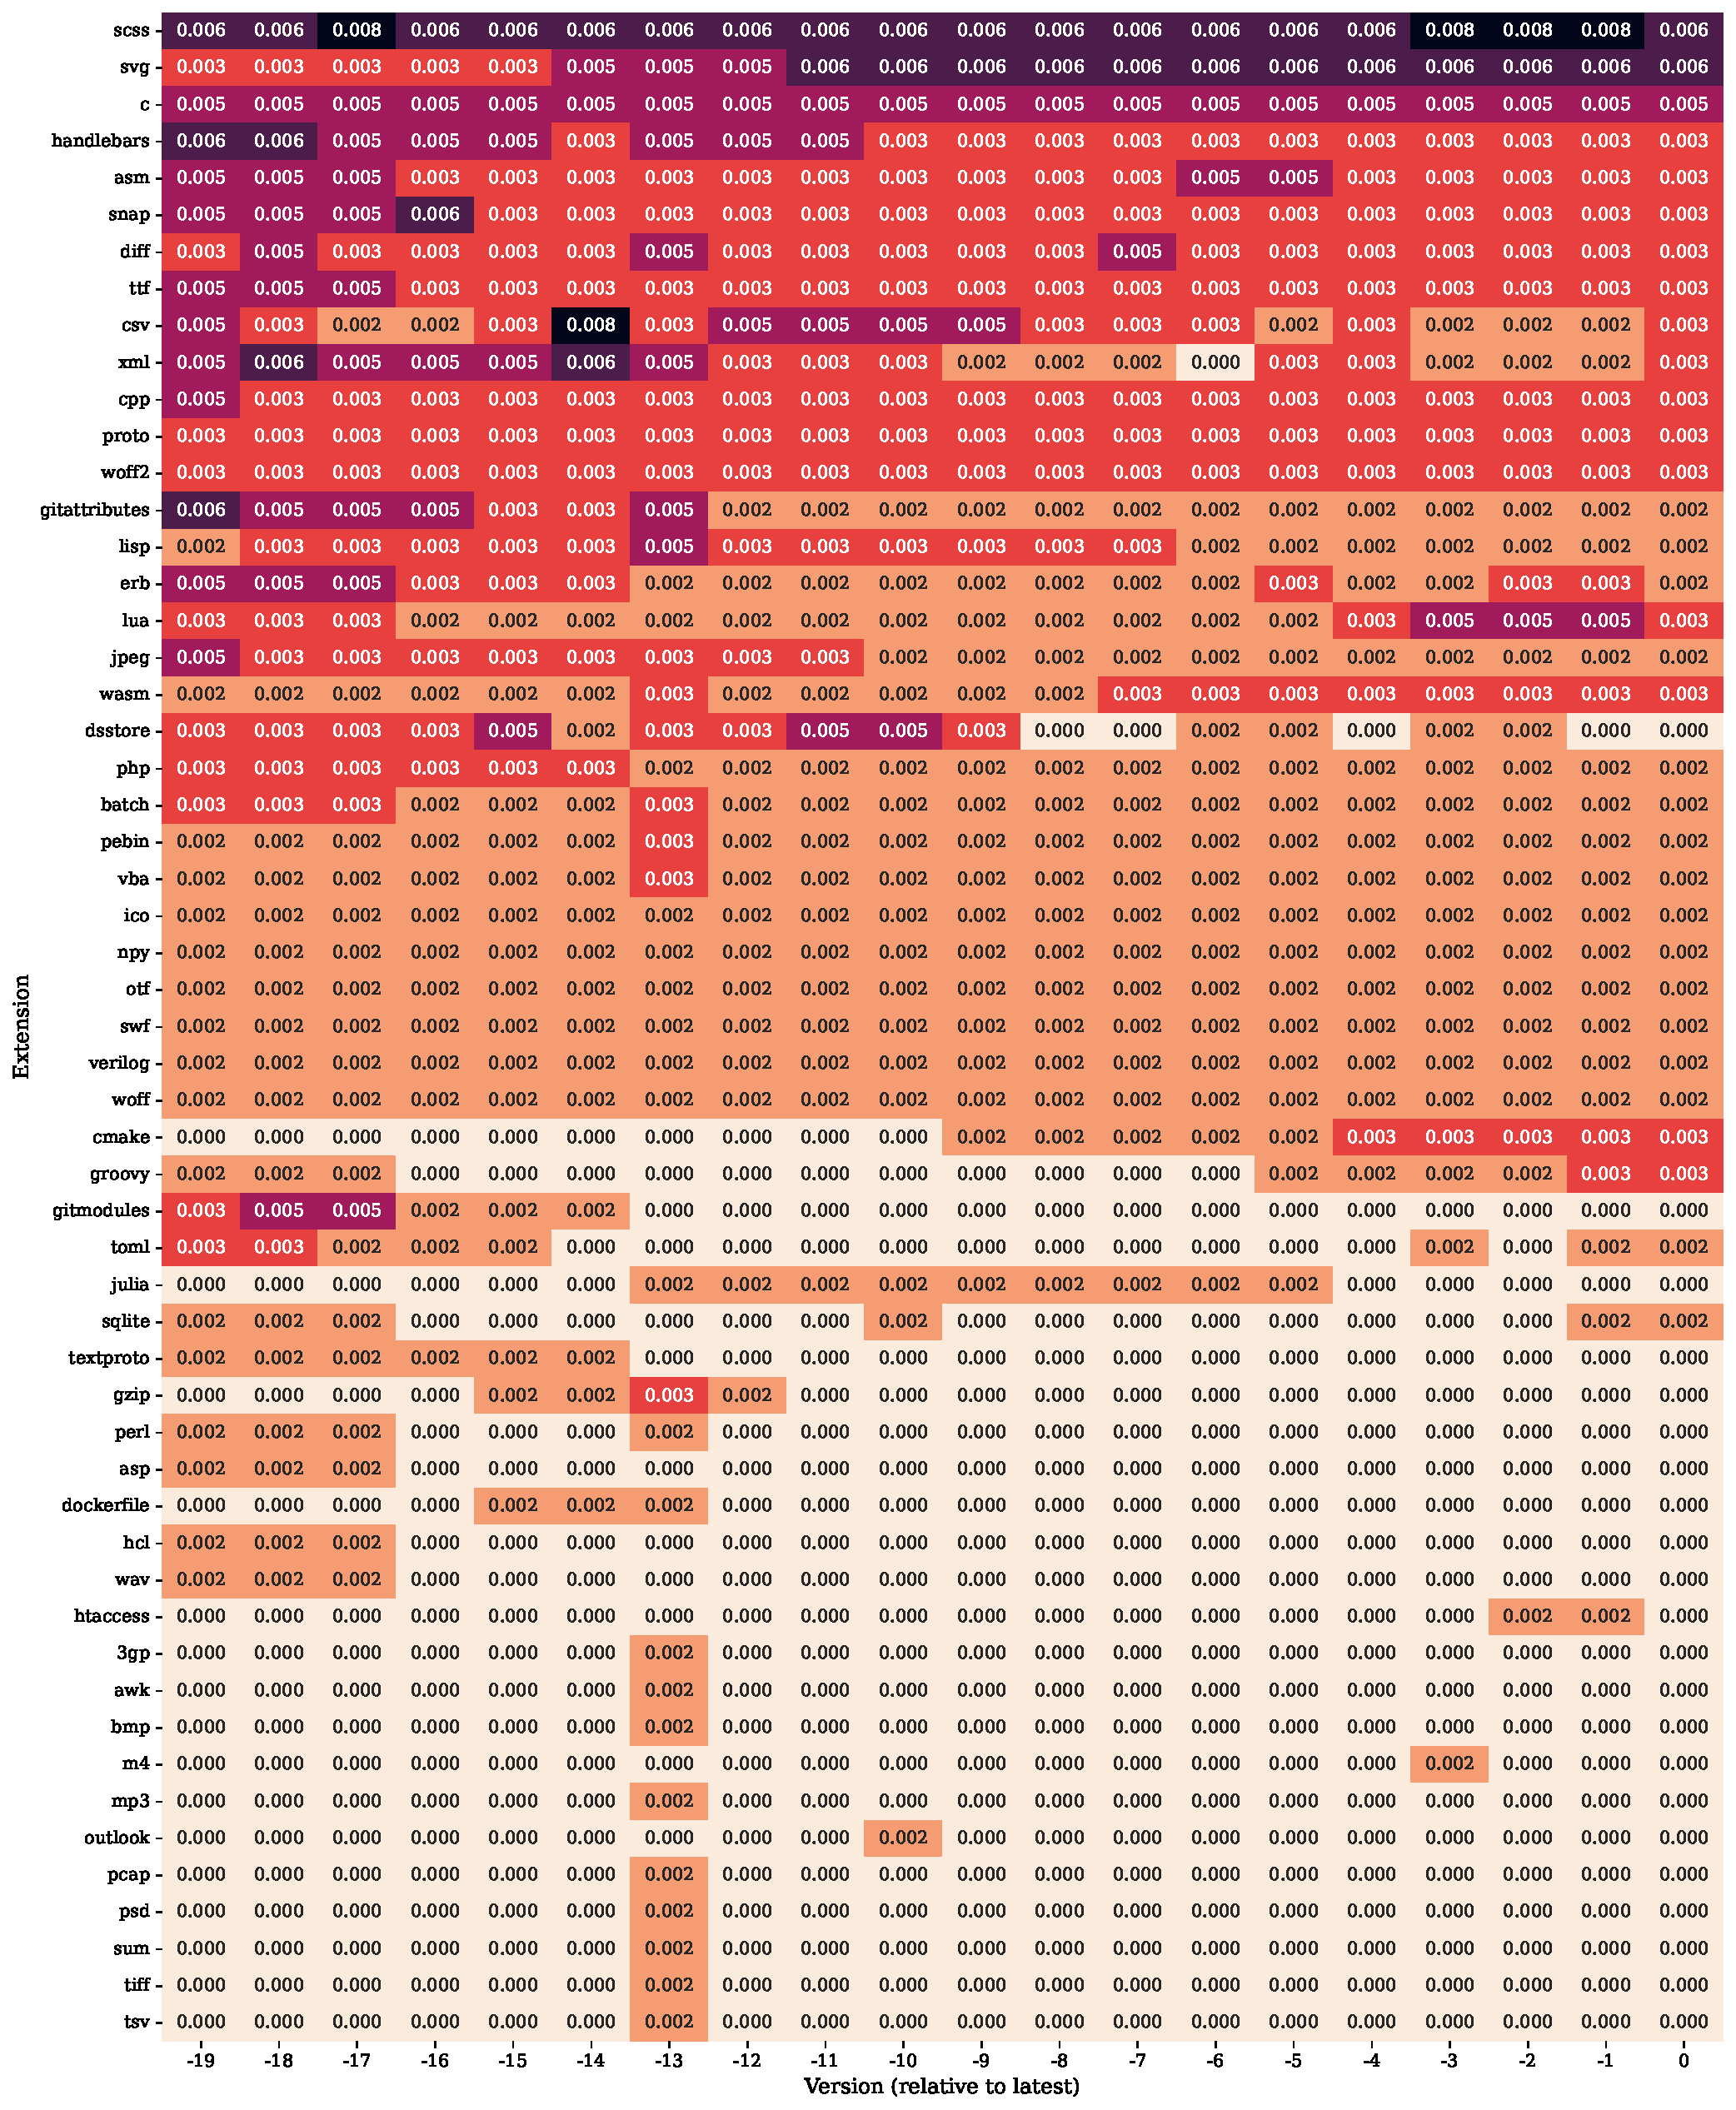
\includegraphics[width=\textwidth]{metrics/filetype/heatmap_rare.pdf}
    \caption{Heatmap for Rare File Types (Outliers)}
    \label{fig:fig1RareFileTypes}
\end{figure}

The extensions shown in \cref{fig:fig1RareFileTypes} (fifty-five in total) are outliers, representing file types present in very few packages.
We analyzed the most interesting extensions and their nature.

\begin{itemize}
    \item \textbf{C and C++}. Three packages, \texttt{sharp}, \texttt{node-addon-api} and \texttt{nan}; contain C and C++ files.
    The \texttt{sharp} package is used for image processing (i.e., resizing, conversion, pixel operations) 
    and relies on the C library libvips to maximize performance and speed~\cite{sharp}.
    To execute C code within Node.js, the use of packages such as \texttt{node-addon-api} (the more modern approach) or \texttt{nan} is required~\cite{node-addon-api, nan}.
    This dependency is necessary because Node.js, being based on JavaScript, cannot natively execute C code.
    These packages act as wrappers, translating calls between the JavaScript environment and the C code.

    \item \textbf{gzip}. Two packages, \texttt{polished} and \texttt{moment-timezone}, included a gzip file by mistake.
    Specifically, the \texttt{polished} package tarball included a \texttt{.yarn} cache directory containing 
    numerous files including \texttt{install-state.gz}, 
    for four consecutive versions (4.0.0-beta.2 to 4.0.3).
    This was removed in version 4.0.4, as reported in the release notes on GitHub~\cite{polished_release_notes}.

    Similarly, \texttt{moment-timezone} (version 0.5.36) erroneously included a temporary folder, \texttt{temp.bac},
    which was entirely unrelated to the package's functionality.
    This folder contained various files types such as gzip, PE, mp3 and psd, 
    and was subsequently removed in the following version.

    \item \textbf{Dockerfile}. A dockerfile appeared in a single package, \texttt{recast}, for three versions (0.21.3 to 0.21.5 included).
    In these versions, the \texttt{.devcontainer} folder was mistakenly included, 
    which contains a dockerfile that configures a container with Node.js and Typescript useful only for maintainers.
    This folder was removed in subsequent versions.

\end{itemize}

\newpage
\subsection{Comparison with Malware Dataset}
\label{sec:analysisFileTypesComparisonMalware}

In attack A (\cref{sec:attackA}), the attacker introduced a malicious Windows \ac{DLL} into the tarball,
which \texttt{Magika} correctly identifies as a \ac{PE} (Pebin, PE Windows executable) file.

As shown in \cref{fig:fig1RareFileTypes}, the Goodware dataset contains two packages with \ac{PE} files: 
\texttt{nodemon} (in all 20 versions) and \texttt{moment-timezone} (in one version).

\begin{itemize}
    \item The \texttt{nodemon} package is a tool that helps develop Node.js based applications 
    by automatically restarting the node application when file changes in the directory are detected~\cite{nodemon}.
    Specifically, it includes \texttt{windows-kill.exe} to ensure signal event (like CTRL+C) work correctly on Windows, 
    for instance, to allow a clean process shutdown.

    \item In contrast, the \texttt{moment-timezone} included a \ac{PE} file by mistake within a temporary folder,
    as previously discussed in \cref{sec:analysisFileTypesGoodware}.

\end{itemize}

Consequently, this metric is efficient in detecting attack A because the malicious versions contain outlier file types.

However, the metric is not indicative for the other three attacks because the malicious versions modify file types that are not outliers, 
such as JavaScript, making them indistinguishable from legitimate versions using this metric alone.